% 2016 全国卷Ⅰ理科第 22 题：圆、弦 CD 与相切的等腰三角形 OAB。
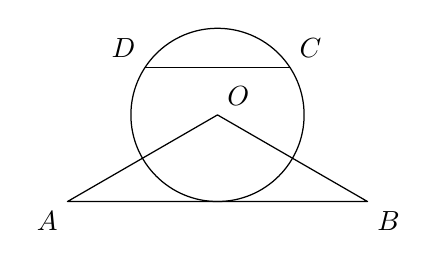
\begin{tikzpicture}[line width=.45pt,line cap=round,line join=round]
  \coordinate (O) at (0,0);
  \coordinate (A) at (-1.905,-1.10);
  \coordinate (B) at (1.905,-1.10);
  \coordinate (D) at (-.919,.605);
  \coordinate (C) at (.919,.605);

  \draw (O) circle[radius=1.10];
  \draw (D)--(C);
  \draw (O)--(A) (O)--(B) (A)--(B);

  \node[above right] at (O) {$O$};
  \node[above left] at (D) {$D$};
  \node[above right] at (C) {$C$};
  \node[below left] at (A) {$A$};
  \node[below right] at (B) {$B$};
\end{tikzpicture}
